\chapter{Vývojové rozhraní}
\label{ch:development}

% TODO: Zkratky MVT, SEO, Framework, XSS, SQL (Injection), SPA, Open-Source, DOM

\section{Frameworky}
\label{sec:dev-framework}
Framework, v jiných slovech struktura nebo kostra, představuje v informatice a softwarovém inženýrství abstraktní koncept poskytující základní stavební kameny pro aplikace s širokým spektrem funkcí. Cílem frameworků je usnadnit vývoj aplikací tím, že nabízejí předem definovanou strukturu, kterou lze dále rozšiřovat o vlastní kód a funkcionalitu. Tímto způsobem umožňují frameworky vývojářům rychleji a efektivněji vytvářet aplikace, což přináší zvýšení produktivity, snížení nákladů na vývoj a hlavně standardizaci kódu mezi vývojáři.

Ve svéře informatiky se frameworky dělí podle jazyku nebo zaměření na aplikace. Máme zde druhy frameworku určených na vývoj webů, rozděleny ny frontend a backend, mobilních aplikací nebo čistě na široký výzkum. \cite{about_framework}

\subsection*{Rozdíl mezi Frameworkem a Knihovnou}
Framework a knihovna jsou dvě často zaměňované koncepce, avšak existují zásadní rozdíly mezi nimi. Knihovna je soubor funkcí nebo tříd, které lze využít při vytváření aplikace. Zajišťuje určitou funkcionalitu, ale vývojář nese odpovědnost za řízení toku aplikace a volání funkcí knihovny.

Naopak framework poskytuje kompletní strukturu aplikace, kde vývojář implementuje pouze specifickou funkcionalitu. Framework tak aktivně řídí tok aplikace a volá konkrétní části kódu, zatímco vývojář se zaměřuje na přizpůsobení těchto specifických částí.

\begin{figure}[H]
    \centering
    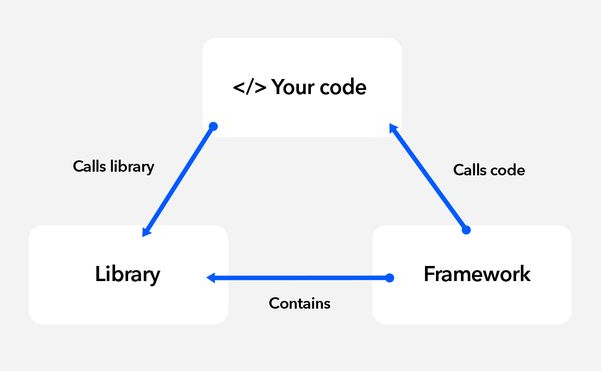
\includegraphics[width=0.6\textwidth]{figures/framework_library_difference}
    \caption{Rozdíl mezi \textit{Frameworkem} a \textit{Knihovnou}. \cite{framework_library_difference}}
    \label{fig:framework_library_difference}
\end{figure}

\subsection*{Model-View-Template vs. Model-View-Controller}
Model-View-Template dále jen jako MVT a Model-View-Controller dále jen jako MVC jsou návrhové vzory, které se široce využívají v softwarovém vývoji webových aplikací. Tyto vzory rozdělují průběh aplikaci do tří propojených částí, kde každá část má svou specifickou roli a odpovědnost. Díky této struktuře je možné izolovat různé části aplikace a tím zvyšovat modularitu, znovu použitelnost a udržitelnost kódu.

V případě MVT je aplikace rozdělena na tři části: \textit{Model}, \textit{View} a \textit{Template}. Model zde reprezentuje datovou strukturu, většinou tedy namapované objekty získané z databáze, případně z jiného zdroje. View (zobrazení) je zodpovědné za přijímání uživatelských požadavků a zobrazování odpovědi od serveru zpět uživateli, v rámci této komunikace reprezentuje určitý most mezi modelem a šablonou. Jako poslední je zde template (šablona), která v tomto případě přijatá data zpracovává do výsledného HTML kódu pomocí speciálních značek určující předem daný formát stránky. Výsledný HTML kód je následně odeslán zpět uživateli.

Na druhé straně MVC, který je často používán ve zbytku frameworku se oproti MVT liší pouze lehce. Model zde stále reprezentuje datovou strukturu, ale View je naopak zodpovědný o pouhé vykreslování dat uživateli. Novým prvkem je zde Controller, který se zaobírá zbylou interakcí uživatele s aplikací, tedy přijímání požadavků, zpracování dat a následné odeslání zpět uživateli. \cite{mvc_mvt_difference}

\begin{figure}[H]
    \centering
    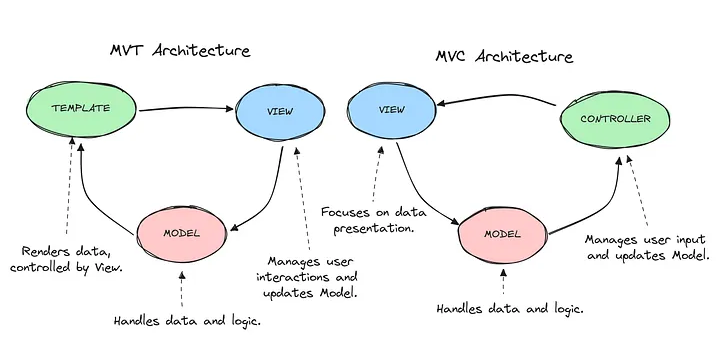
\includegraphics[width=1.0\textwidth]{figures/mvc_mvt_difference}
    \caption{Rozdíl mezi \textit{Model View Template} a \textit{Model View Controller} návrhovými vzory. \cite{mvc_mvt_difference_img}}
    \label{fig:mvc_mvt_difference}
\end{figure}

\subsection{Django}
\label{subsec:dev-framework-django}

Django je výkonným open-source frameworkem určeným pro vývoj robustních a lehce škálovatelných webových aplikací v programovacím jazyce Python. Od svého veřejného uvedení v roce 2005, pojmenovaného po slavném kytaristovi Django Reinhardtovi, získal popularitu díky své schopnosti urychlit vývoj a poskytnout bezpečné a efektivní nástroje pro tvorbu webových aplikací.

Framework Django přistupuje k architektuře webových aplikací pomocí návrhového vzoru Model-View-Template (MVT), což představuje alternativu k tradičnímu přístupu Model-View-Controller (MVC). Tato struktura usnadňuje komunikaci mezi datovým modelem, prezentační vrstvou a šablonami pro serverové vykreslování.

V oblasti vývoje uživatelského rozhraní Django nabízí šablonovací jazyk (DTL), který umožňuje vytvářet dynamická a daty řízená uživatelská rozhraní. To je zvláště užitečné pro aplikace, které kladou důraz na optimalizaci pro vyhledávače (SEO) a vyžadují komplexní logiku na straně serveru. DTL umožňuje vývojářům vytvářet stránky s dynamickým obsahem, který je generován ještě před odesláním HTML kódu ze serveru.

V situacích, kde je potřeba dosáhnout interaktivity uživatele s rozhraním, je možné rozšířit Django o JavaScriptové knihovny nebo volit jiný framework specializovaný na frontendový vývoj. To umožňuje vysoce flexibilní přístup k vytváření moderních a interaktivních webových aplikací. \cite{about_django}.

\subsection{React}
\label{subsec:dev-framework-react}

React je významná JavaScriptová knihovna určená pro vytváření uživatelských rozhraní, především na straně klienta. Vyvinutá firmou Facebook, React využívá virtuální DOM k efektivní aktualizaci komponent a podporuje deklarativní syntaxi pro tvorbu interaktivních uživatelských rozhraní. Je široce používán pro vývoj jednostránkových aplikací (SPA), kde je klíčová potřeba dynamických aktualizací.

React vyniká v poskytování responzivního a interaktivního uživatelského přístupu, což z něj činí oblíbenou volbu pro moderní webový vývoj. Jeho komponentový přístup umožňuje rozdělit uživatelské rozhraní do znovupoužitelných částí, což zjednodušuje správu a údržbu kódu. Využívá návrhový vzor \textit{Model-View-Controller}. \cite{about_react}

\subsection{Angular}
\label{subsec:dev-framework-angular}
Angular je populární open-source framework pro vývoj webových aplikací. Je sponzorován a udržován převážně společností Google a vyniká díky široké komunitě a schopnosti řešit výzvy spojené s vývojem jednostránkových aplikací (SPA). Angular je postaven na jazyce TypeScript a využívá komponentovou architekturu pro tvorbu uživatelských rozhraní.

Jednou z klíčových vlastností Angularu je jeho komplexní systém modulů a komponent, který usnadňuje organizaci a správu kódu. Angular používá návrhový vzor \textit{Model-View-Controller} (MVC) a klade důraz na dvoucestný data-binding, což znamená, že změny v modelu automaticky odrážejí změny v vykreslování a naopak.

Framework obsahuje mnoho vestavěných funkcí, jako například modulární routování, HTTP služby pro komunikaci se serverem, a nástroje pro testování. Angular také poskytuje kompletní sadu nástrojů pro správu stavu aplikace. \cite{about_angular}

\subsection{Laravel}
\label{subsec:dev-framework-laravel}
Laravel je moderní open-source PHP framework, který je určený pro vývoj webových aplikací. Tento framework vytvořil Taylor Otwell a byl poprvé vydán v roce 2011. Vyniká díky své jednoduchosti, efektivitě a schopnosti urychlit vývoj aplikací. Laravel využívá návrhový vzor \textit{Model-View-Controller} (MVC) a poskytuje mnoho vestavěných funkcí, jako například routování, šablonovací systém, a nástroje pro správu databáze.

Mezi jednu z jeho klíčových vlastností patří Eloquent ORM, což je moderní implementace Active Record návrhového vzoru, který umožnuje jednoduše pracovat s namapovanými objekty z databáze jako s obyčejnými PHP objekty. Jako framework Django obsahuje šablonovací systém Blade, které je jednoduchý a efektivní pro vytváření dynamických uživatelských rozhraní. Další výhodou jsou zabudované mechanismy pro zabezpečení aplikace, jako například ochrana proti Cross-Site Scripting (XSS) a SQL Injection útokům. \cite{about_laravel}

\subsection{Vue.js}
\label{subsec:dev-framework-vuejs}
Vue.js je moderní JavaScriptový framework určený pro vývoj uživatelského rozhraní webových aplikací. Jeho největší výhodou je snadná flexibilita a jednoduchá intergrace s již existujícími projekty. Vue.js byl poprvé vydán v roce 2014 a od této doby získal velkou popularitu díky své schopnosti urychlit vývoj a poskytnout efektivní nástroje pro tvorbu moderních webových aplikací.

Jedním z klíčových prvků Vue.js je reaktivní datová vrstva, která umožňuje snadná sledování a aktualizaci dat. Framework využívá jednosměrný datový tok, což znamená, že veškeré změny v datech jsou automaticky aktualizovány v uživatelským rozhraní. Toto chování usnadňuje sledování stavu aplikace a vytváření dynamických a interaktivních uživatelských rozhraní.

Vue.js je navržen ohledem na progresivitu, což znamená, že ho lze snadno a postupně intergrovat do existujícího projektu a nijak tak nenarušit jakoukoliv funkčnost. Při této integraci lze jednoduše rozdělit aplikaci do Frontend části, reprezentovanou Vue.js a backend části, která může být reprezentována například frameworkem Django. \cite{about_vuejs}

\subsection{Svelte}
\label{subsec:dev-framework-svelte}
Svelte je jedním z inovativních JavaScriptových frameworků, který se zaměřuje na efektivní kompilací v ranné fázi build procesu, což přináší nový pohled na vývoj uživatelské rozhraní. Zatímco tradiční frameworky provadějí většinu práce na straně klienta nebo serveru za běhu, Svelte přesouvá tuto činnost do fáze komiplace, čímž mnohonásobně zlepšuje výkon a optimalizuje výslednou velikost kódu.

Klíčovým konceptem Svelte je štěpení kódu do komponent, které jsou více než pouze části uživatelské rozhraní. Tyto komponenty obsahuje více než prezentační logiku, definují také jak se má komponent chovat a jaké akce má provádět pod určitými podmínkami. Tento přístup tak umožnuje jednoduše eliminovat zbytečný nebo duplicitní kód ve fázi kompilace, jako dělají například \textit{C++ kompilátory}.

Pro plné využití tohoto frameworku, je nutné jeho rozšíření o backendovou část, která bývá zodpovědná za zpracování dat a komunikaci se serverem. Tato část může být reprezentována například jedním s frameworků zmíněných výše. \cite{about_svelte}

\subsection{Shrnutí a Srovnání}
\label{subsec:dev-framework-comparison}
Srovnání frameworku zmíněných výše dosahuje celkového závěru, že každý z ních má své výhody a nevýhody. Pomocí každého frameworku nebo jejich kombinací lze vytvořit moderní a efektivní webové aplikace, které by splňovaly mnoho požadavků ze strany efektivního vývoje, výkonu a bezpečnosti.
Každý z frameworků používá jiný jazyk, ať to je buď Python, JavaScript nebo PHP, což může být klíčové pro jeho výběr vzhledem k projektu. Dalším faktorem je dokumentace, komunita a dostupnost nástrojů, které mohou být klíčové pro rychlý vývoj a řešení problémů.

\section{Zpracování požadavku}
\label{sec:dev-request-processing}

% TODO: Přidat obrázek, který bude znázorňovat rozdíly mezi SSR, CSR a Hybridním vykreslováním
% TODO: Zkracený popis

\subsection{Client-Side Rendering}
\label{subsec:dev-request-processing-client-side-rendering}
Server odesílá uživateli kompletní zdrojový kod, kompilace a vykreslení probíhá až na straně klienta.
% TODO:

\subsection{Server-Side Rendering}
\label{subsec:dev-request-processing-server-side-rendering}
Server předvykresluje stránku a odesílá ji uživateli jako kompletní HTML kód.
% TODO:

\subsection{Hybrid Rendering}
\label{subsec:dev-request-processing-hybrid-rendering}
Kombinace obou přístupů, kde se stránka předvykreslí na serveru a následně se na straně klienta probíhá další dynamické aktualizace.
% TODO:

\section{Technologie}
\label{sec:dev-technology}

\subsection{Šablonování}
\label{subsec:dev-technology-templating}

Šablonování v rámci Djanga představuje klíčovou technologii pro vytváření dynamických uživatelských rozhraní webových aplikací, kde jeho hlavním účelem je oddělit prezentaci dat (Presentation Layer) od logiky zpracování (Business Layer), což vede k zvýšení modularizace a udržitelnosti kódu. Tento systém umožňuje vývojářům definovat strukturu a vzhled webových stránek pomocí šablon, které se na sebe mohou vázat, rozšiřovat se. Tyto šablony obsahují statický HTML kód spolu s vloženými proměnnými, filtry a řídícími strukturami, které se později zpracovávají na serveru a následně odesílají uživateli.

Mezi hlavní výhody používání šablon patří:
\begin{enumerate}
    \item \textbf{Oddělení Prezentace a Logiky:} Šablonování umožňuje jasně a jednoduše oddělit prezentaci dat (HTML kód) od logiky zpracování těchto dat (Python nebo JavaScript). Toto rozdělení zvyšuje čitelnost a spravovatelnost kódu.
    \item \textbf{Hermetická Integrace s Frameworkem:} Django šablonovací systém je plně integrován s ostatními komponentami frameworku, což usnadňuje přístup k databázím, formulářům a dalším funkcím Djanga přímo ze šablon za pomocí speciálních značek a filtrů.
    \item \textbf{Podpora Dynamických Dat:} Díky použití proměnných a filtrů umožňuje šablonovací systém dynamicky zobrazovat data na stránkách. To je klíčové pro vytváření interaktivních a daty řízených uživatelských rozhraní.
    \item \textbf{Zabezpečení:} Systém frameworku obsahuje mechanismy pro prevenci útoků jako Cross-Site Scripting (XSS), Form tampering, SQL injection a další. Tato zabezpečení jsou automaticky aplikována na šablony, což zvyšuje bezpečnost aplikace.
\end{enumerate}

Celkově lze konstatovat, že technologie šablonování v Djangu přispívá k efektivnímu a strukturovanému vývoji webových aplikací, usnadňuje spolupráci mezi vývojáři a designéry a zvyšuje obecnou robustnost aplikace.

\subsection{Balíčkovací systémy}
\label{subsec:dev-technology-package-managers}

\subsubsection{NPM}
\label{subsubsec:dev-technology-package-managers-npm}

\subsubsection{Yarn}
\label{subsubsec:dev-technology-package-managers-yarn}

\subsubsection{PIP}
\label{subsubsec:dev-technology-package-managers-pip}

\endinput